% !TEX program = xelatex
\documentclass[hyperref,a4paper,UTF8]{ctexart}

\usepackage[left=2.50cm, right=2.50cm, top=2.50cm, bottom=2.50cm]{geometry}

\usepackage[unicode=true,colorlinks,urlcolor=blue,linkcolor=blue,bookmarksnumbered=true]{hyperref}
\usepackage{latexsym,amssymb,amsmath,amsbsy,amsopn,amstext,amsthm,amsxtra,color,bm,calc,ifpdf}
\usepackage{graphicx}
\usepackage{enumerate}
\usepackage{fancyhdr}
\usepackage{listings}
\usepackage{multirow}
\usepackage{makeidx}
\usepackage{xcolor}
\usepackage{fontspec}
\usepackage{subfigure}
\usepackage{hyperref}
\usepackage{pythonhighlight}

\pagestyle{fancy}
\fancyhead[L]{}
\fancyhead[C]{\fangsong 转角双层石墨烯物理性质研究}
\fancyhead[R]{}

\renewcommand{\abstractname}{\textbf{\large {摘\quad 要}}} % 更改摘要二字的样式


\title{\textbf{{石墨烯掺杂原神的性质研究}}}
\author{
\kaishu\normalsize
姓名\ \underline{{一二三四 }
} \qquad
学号\ \underline{114514} \qquad
院系\ \underline{提瓦特大陆}
}
\date{} % 留空,不显示日期


\begin{document}

\begin{figure}
    \centering
    
\includegraphics[width=0.75\textwidth]{figures/swust.png}
\end{figure}

\maketitle

\begin{abstract}

石墨烯作为一种新奇的二维材料,自被发现以来一直受到科研人员的关注,2018年曹原在一篇nature中给我们带来了转角石墨烯(twisted bilayer graphene,TBG)。由于转角体系的可调控性及其衍生出的平带强关联物理,为全新的低能物理强关联体系研究开辟了新方向。本文简要回顾了转角双层石墨烯的理论推导及其实验验证,论述了其超导特性,为后续继续研究二维转角材料体系提供了范例

\end{abstract}

\

\tableofcontents

\thispagestyle{empty} % 当前页不显示页码
\newpage


\section{引言}

2018年的春天,曹原以魔角(约1.1°)双层石墨烯的工作在顶级期刊Nature上背靠背发表了两篇文章,2020年5月,曹原和他的导师及合作者在Nature上报道了转角双层-双层石墨烯以及利用nano-SQUID(纳米超导量子干涉仪)表征转角双层石墨烯中角度非均一性问题的两项相关工作,将转角电子学领域推向了又一个高潮。实际上,自2018年3月魔角双层石墨烯问世以来,和转角二维材料有关的科研工作至今已经有超过13项发表在Nature和Science两大顶级期刊上。通俗的讲,曹原他们研究的工作在科学上的术语称为:摩尔超晶格。摩尔超晶格本质上是两套空间分布相近的格子叠加在一起相互干涉形成的一套低频、长周期的新格子。通俗地讲,两套格子在空间堆叠上,时而密集,时而稀疏,这种疏密的周期分布形成了所谓的摩尔条纹。摩尔条纹在我们的日常生活中常常可以见到。例如,用手机拍摄电脑屏幕时,生成的照片上常常伴随着肉眼可见的畸形条纹。这是因为电脑屏幕的发光元件阵列和手机摄像头里的CCD或CMOS感光元件组成了两套相近的格子,它们相互叠加形成了摩尔条纹。摩尔条纹的图样和格子间的转角密切相关。感兴趣的童鞋,可以在身边寻找两套相同的格子(譬如窗纱),手动旋转它们,观察摩尔条纹的变化。尽管摩尔条纹给电子显示和拍摄带来不小麻烦,科学家却想到了利用二维材料中的摩尔条纹去观察新的物理现象。只需要将窗纱换成晶格接近或者相同的两层二维材料,并且小角度堆叠在一起,便可以构筑二维的微观摩尔条纹,即二维摩尔超晶格(曹原便是将窗纱换成了两层石墨烯,两层石墨烯间旋转约1.1°)。除此以外,二维材料,顾名思义,它的厚度薄到可以将之视为二维极限。常见的二维材料包括石墨烯(石墨的基本组成单元,只含有一层碳原子,碳原子按照六角蜂窝状周期排列)、薄层过渡金属硫化物(如二硫化钼MoS2等,通常是良好的半导体材料)。由于二维材料太薄,两层二维材料的界面便能代表整体的性质。因此,二维材料被视为摩尔超晶格研究的最合适载体之一。在现实的材料中,电子之间可以靠静电相互作用(库伦作用力)彼此关联在一起,它们的多体关联往往诱导出奇特的物理性质。譬如,在铜基的陶瓷材料中,科学家发现它的超导转变温度可以大幅提升至液氮的沸点温度以上,因此具有很高的实用价值(中国科学家在这个领域做出了突出贡献)。实现室温的超导转变,对未来的能源和交通发展将会产生革命性影响。因此,在基础物理研究上,寻找这样的强关联体系并挖掘其中的物理奥秘,一直是一项非常重大的课题。而转角摩尔超晶格便是一个很好的多体关联体系。在2011年,尽管当时人们已经认识到将两层石墨烯以一定的转角堆叠起来,可以形成二维摩尔超晶格,并带来新的物理现象。但是,直到美国的理论物理学家Allan H. MacDonald教授和Rafi Bistritzer博士计算出转角为1.1°的双层石墨烯超晶格中电子的速度会大幅降低,人们才开始逐渐认识到1.1°转角双层石墨烯超晶格蕴含了丰富的多体强关联物理。在理论预测之后,实验科学家开始尝试利用各种方法去制备这样的转角石墨烯超晶格样品,并观测其中的多体物理现象。2018年,曹原和他的导师Pablo Jarillo-Herrero教授率先实现了魔角双层石墨烯样品的制备,并在低温下(约零下270℃)观测到金属态到绝缘态的转变。令人震惊的是,他们意外地发现,如果向转变后的绝缘态添加一定量的电子,居然能诱导出超导现象!这种行为和我们上文介绍的铜基超导体很像。因此,魔角双层石墨烯对于认识高温超导机制具有重要作用。本篇文章旨在回顾这一系列发现,为从转角双层石墨烯出发认识高温超导机制做一些简单的介绍。

\section{理论推导}
我们主要以转角石墨烯作为例子展开本文,故在细致推导之前,我们先对石墨烯及其转角体系的参数进行统一定义。我们采取下图所示的原胞选取:即$\mathbf{a}_1 = \frac{a}{2} ( \sqrt{3}, 3),\,\mathbf{a}_2 = \frac{a}{2} (-\sqrt{3}, 3)$,其中sublattice相对原胞原点的位矢定义为:$\delta^A = 0,\, \delta^B = \frac{1}{3}( \mathbf{a}_1 + \mathbf{a}_2 )$
\begin{figure}[h]
	\centering
	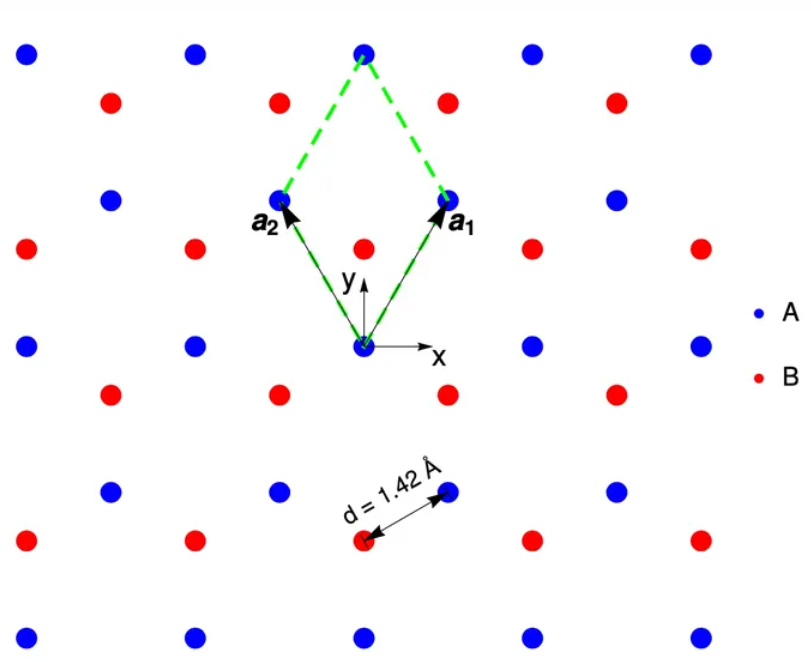
\includegraphics[scale=0.6]{figures/gra.png}
	\caption{石墨烯实空间晶格示意图}
\end{figure}
对应的倒空间单位矢量为:$\mathbf{b}_1 = \frac{2\pi}{3a}(\sqrt{3}, 1),\,\mathbf{b}_2 = \frac{2\pi}{3a}(-\sqrt{3}, 1)$,Brillouin Zone(BZ)高对称点坐标:$\mathbf{K} = \frac{1}{3}(\mathbf{b}_1 - \mathbf{b}_2)$。定义real space基底与Fourier space基底的变换关系:$| \mathbf{R}, \alpha\rangle = \frac{1}{\sqrt{N}}\sum_{\mathbf{k} \in BZ} e^{-i \mathbf{k} \cdot (\mathbf{R} + \delta^\alpha)} | \mathbf{k}, \alpha\rangle$,$| \mathbf{k}, \alpha \rangle = \frac{1}{\sqrt{N}}\sum_{\mathbf{R} \in \Lambda} e^{i \mathbf{k} \cdot (\mathbf{R} + \delta^\alpha)} | \mathbf{R}, \alpha\rangle$,其中$\Lambda$代表由$\mathbf{a}_{1,2}$为基矢展成的所有site,类似定义$\Lambda^*$为倒空间中由$\mathbf{b}_{1,2}$为基矢展成的所有site。

\subsection{动量空间连续模型}
一般而言,只有满足特殊角度取值的转角体系,才能恰好形成更大的超胞,从而有周期晶格、Moire BZ等相关的后续研究,这种特殊的构型被称为commensurate configuration,而其余不能在real space形成有限大小超胞的构型则被称为incommensurate configuration。
\begin{figure}[h]
	\centering
	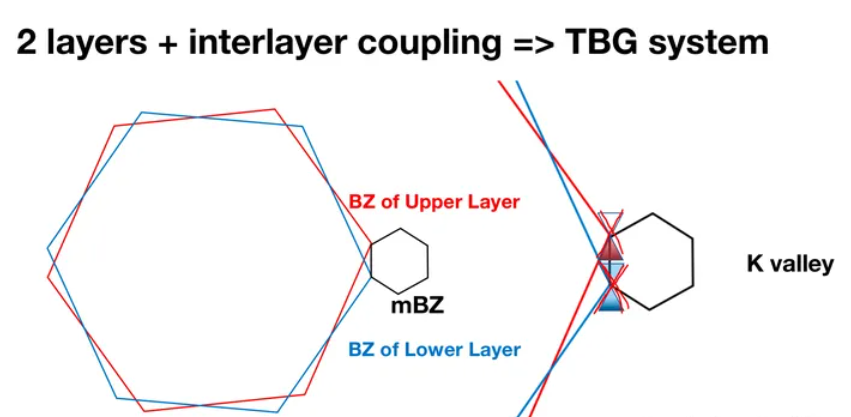
\includegraphics[scale=0.6]{figures/layer.png}
\end{figure}

我们可以简单认为在小角度时,我们总可以认为构型是commensurate的,其Moire BZ可以看做是由两层BZ的K点间的连线$\mathbf{K}_- - \mathbf{K}_+$作为六角Moire BZ的$\mathbf{K}_M - \mathbf{K}_M'$形成的。从而我们有BZ和Moire BZ的尺寸关系:$|\mathbf{K}_M| = 2 \sin \frac{\theta}{2} |\mathbf{K}|$。从而根据real space与reciprocal space的倒易关系,可以推算real space的supercell lattice constant:$a_M = \frac{a}{2 \sin \frac{\theta}{2}}$,对于N维单体波函数空间的体系,real space超胞内含原子多了$(2 \sin \frac{\theta}{2})^2$倍,则对应的reciprocal space的mBZ内的面积对应的少了$(2 \sin \frac{\theta}{2})^2$倍,总的自由度数量不变。

\
\subsection{构建哈密顿量}
单层哈密顿量即Dirac cone,并通过人为superlattice选取和BZ的划分,使原先分布在BZ能带折叠到mBZ中。真正贡献了superlattice coupling的是interlayer coupling,即层间的跃迁矩阵元:

$$\begin{aligned} & \langle \mathbf{k}'_{-l}, \alpha' | \hat{H}_{int} | \mathbf{k}_{l}, \alpha \rangle \\ & = \left( \frac{1}{\sqrt{N}}\sum_{\mathbf{R}'_{-l} \in \Lambda_{-l}} e^{-i \mathbf{k}'_{-l} \cdot (\mathbf{R}'_{-l} + \delta^{\alpha'}_{-l})} \langle \mathbf{R}'_{-l}, \alpha' | \right) \hat{H}_{int} \left( \frac{1}{\sqrt{N}}\sum_{\mathbf{R}_l \in \Lambda_l} e^{i \mathbf{k} \cdot (\mathbf{R}_l + \delta^\alpha_l)} | \mathbf{R}_l, \alpha \rangle \right) \\ & = \frac{1}{N} \sum_{\mathbf{R}'_{-l} \in \Lambda_{-l}} \sum_{\mathbf{R}_l \in \Lambda_l} e^{-i \mathbf{k}'_{-l} \cdot (\mathbf{R}'_{-l} + \delta^{\alpha'}_{-l})} e^{i \mathbf{k} \cdot (\mathbf{R}_l + \delta^\alpha_l)} \langle \mathbf{R}'_{-l}, \alpha' |\hat{H}_{int} | \mathbf{R}_l, \alpha \rangle \end{aligned}$$

其中$\langle \mathbf{R}'_{-l}, \alpha' |\hat{H}_{int} | \mathbf{R}_l, \alpha \rangle$为real space的interlayer coupling,满足平移对称性:

$$\begin{aligned} \langle \mathbf{R}'_{-l}, \alpha' |\hat{H}_{int} | \mathbf{R}_l, \alpha \rangle & = t_{\perp} (\mathbf{R}'_{-l} + \delta^{\alpha'}_{-l} - \mathbf{R}_l - \delta^{\alpha}_{l} ) \\ & = \int_{\mathbb{R}^2} \frac{d^2 \mathbf{q}}{(2\pi)^2} t_\perp (\mathbf{q}) e^{i \mathbf{q} \cdot ( \mathbf{R}'_{-l} + \delta^{\alpha'}_{-l} - \mathbf{R}_l - \delta^{\alpha}_{l} )} \end{aligned}$$

对积分进行粗粒化处理可以改为求和:

$$\int_{\mathbb{R}^2} d^2 \mathbf{q} = \sum_{\mathbf{q} \in \{( \frac{2\pi n_x}{N_x a_x}, \frac{2\pi n_y}{N_y a_y} )\}} \Delta q_x \Delta q_y = \sum_{\mathbf{q} \in \Delta q^2 \mathbb{Z}^2} \frac{2\pi}{N_x a_x} \frac{2\pi}{N_y a_y} = \frac{(2\pi)^2}{N A_{u.c.}} \sum_{\mathbf{q} \in \Delta q^2 \mathbb{Z}^2}$$

其中,$A_{u.c.} = a_x a_y$为原胞面积(此处强行使用矩形倒空间晶格,但对于六角情形同样适用)。从而有
$$\langle \mathbf{R}'_{-l}, \alpha' |\hat{H}_{int} | \mathbf{R}_l, \alpha \rangle = \frac{1}{N} \sum_{\mathbf{q}} \frac{t_\perp (\mathbf{q})}{A_{u.c.}} e^{i \mathbf{q} \cdot ( \mathbf{R}'_{-l} + \delta^{\alpha'}_{-l} - \mathbf{R}_l - \delta^{\alpha}_{l} )}$$

代入momentum space coupling矩阵元有:

$$\begin{aligned} & \langle \mathbf{k}'_{-l}, \alpha' | \hat{H}_{int} | \mathbf{k}_{l}, \alpha \rangle \\ & = \frac{1}{N} \sum_{\mathbf{R}'_{-l} \in \Lambda_{-l}} \sum_{\mathbf{R}_l \in \Lambda_l} e^{-i \mathbf{k}'_{-l} \cdot (\mathbf{R}'_{-l} + \delta^{\alpha'}_{-l})} e^{i \mathbf{k}_l \cdot (\mathbf{R}_l + \delta^\alpha_l)} \langle \mathbf{R}'_{-l}, \alpha' |\hat{H}_{int} | \mathbf{R}_l, \alpha \rangle \\ & = \sum_{\mathbf{q}} \frac{t_\perp (\mathbf{q})}{A_{u.c.}} \left( \frac{1}{N} \sum_{\mathbf{R}' \in \Lambda_{-l}} e^{i (\mathbf{q} - \mathbf{k}'_{-l}) \cdot \mathbf{R}'_{-l}} \right) \left( \frac{1}{N} \sum_{\mathbf{R} \in \Lambda_l} e^{- i (\mathbf{q} - \mathbf{k}_l) \cdot \mathbf{R}_l} \right) e^{i (\mathbf{q} - \mathbf{k}'_{-l}) \cdot \delta^{\alpha'}_{-l}} e^{-i (\mathbf{q} - \mathbf{k}_l) \cdot \delta^{\alpha}_l} \\ & = \sum_{\mathbf{q}} \frac{t_\perp (\mathbf{q})}{A_{u.c.}} \sum_{\mathbf{G}'_{-l} \in \Lambda^*_{-l}} \delta_{\mathbf{q} - \mathbf{k}'_{-l},\mathbf{G}'_{-l}} \sum_{\mathbf{G}_l \in \Lambda^*_{l}} \delta_{\mathbf{q} - \mathbf{k}_l,\mathbf{G}_l} e^{i (\mathbf{q} - \mathbf{k}'_{-l}) \cdot \delta^{\alpha'}_{-l}} e^{-i (\mathbf{q} - \mathbf{k}_l) \cdot \delta^{\alpha}_l} \\ & = \sum_{\mathbf{q}} \frac{t_\perp (\mathbf{k}_l + \mathbf{G}_l)}{A_{u.c.}} \sum_{\mathbf{G}'_{-l} \in \Lambda^*_{-l}} \delta_{\mathbf{q} - \mathbf{k}'_{-l},\mathbf{G}'_{-l}} \sum_{\mathbf{G}_l \in \Lambda^*_{l}} \delta_{\mathbf{q} - \mathbf{k}_l,\mathbf{G}_l} e^{i \mathbf{G}'_{-l} \cdot \delta^{\alpha'}_{-l}} e^{-i \mathbf{G}_l \cdot \delta^{\alpha}_l} \\ & = \sum_{\mathbf{G}' \in \Lambda^*} \sum_{\mathbf{G} \in \Lambda^*} \frac{t_\perp (\mathbf{k}_l + \mathbf{G}_l)}{A_{u.c.}} e^{i \mathbf{G}' \cdot \delta^{\alpha'}} e^{-i \mathbf{G} \cdot \delta^{\alpha}} \delta_{\mathbf{k}'_{-l} + \mathbf{G}'_{-l} , \mathbf{k}_l + \mathbf{G}_l} \end{aligned}$$
\
\subsection{石墨烯魔角条件}
由于平带的条件为renormalized Fermi velocity变为0,即magic angle condition:$w_1 = \frac{1}{\sqrt{3}}$。这是无量纲情形下的结果,如果回到有量纲的情形,则magic angle condition为:$w_1 = \frac{t_\perp (|\mathbf{K}|)}{A_{u.c.}} / \hbar v_F |\mathbf{K_M}| = \frac{t_\perp (|\mathbf{K}|)}{2 A_{u.c.} \hbar v_F |\mathbf{K}| \sin(\theta/2)} = \frac{1}{\sqrt{3}}$,代入具体的参数:$t_\perp (|\mathbf{K}|) \approx 0.58 eV Å ^2$,由graphene lattice constant a = 1.42 Å可以算出$A_{u.c.} = \frac{3\sqrt{3}}{2}a^2 = 5.238 Å^2$,$|\mathbf{K}| = \frac{4\pi}{3a} = 1.703 Å^{-1}$,graphene的Fermi velocity:$\hbar v_F = 5.965 eV Å$,小角度近似下$2\sin(\theta/2) \approx \theta$,从而magic angle对应了:$\theta_{magic} = \frac{\sqrt{3}t_\perp (|\mathbf{K}|)}{A_{u.c.}\hbar v_F |\mathbf{K}|} = \frac{\sqrt{3} \times 0.58 eV Å^2}{5.238 Å^2 \times 5.965 eV Å \times 1.703 Å^{-1}}$,可得到:$\theta_{magic} = 0.0188 \text{rad} \approx 1.1^\circ$,这便是著名的转角石墨烯的魔角条件,与实验上在$1.1^\circ$附近观测到平带基本一致。虽然仅在一点出Fermi velocity降为0,但事实上此时整个mBZ内的能带都十分平,Bernevig等人进一步通过$\Gamma_M-centered model$分析了能带不仅在$K_M$附近费米速度降为0,而且在$\Gamma_M$附近能量也接近0,而Ashvin等人在"Origin of Magic Angles in Twisted Bilayer Graphene"一文中则用了chiral TBG model,给出了TBG平带与Landau Level的对应,这从另一方面说明了Magic Angle regime以及平带出现的必然性,也为TBG等Moire体系中整数、分数量子霍尔效应的研究提供了motivation。
\
\section{实验观测}
普林斯顿大学领导的一个科学家团队对精确的微观基础进行了成像,这些基础负责在一种称为魔角扭曲双层石墨烯(MATBG)的材料中观察到的许多量子相。这种非凡的材料由以二维六边形图案排列的碳原子扭曲层组成,近年来一直处于物理学研究的前沿,特别是在凝聚态物理学中。研究人员首次能够专门捕获相互作用电子的微观行为的前所未有的精确可视化,这些相互作用电子产生了MATBG的绝缘量子相。此外,通过使用新颖和创新的理论技术,他们能够解释和理解这些行为。他们的研究发表在《自然》杂志上。扭曲双层石墨烯的惊人特性于2018年由麻省理工学院(MIT)的Pablo Jarillo-Herrero及其团队首次发现。他们表明这种材料可以是超导的,一种电子在没有任何阻力的情况下自由流动的状态。这种状态对我们的许多日常电子产品至关重要,包括用于MRI和粒子加速器的磁铁,以及用于构建量子计算机的量子比特(称为量子比特)的制造。下图给出了扭曲双层石墨烯的扫描隧道显微镜图像。

\begin{figure}[h]
	\centering
	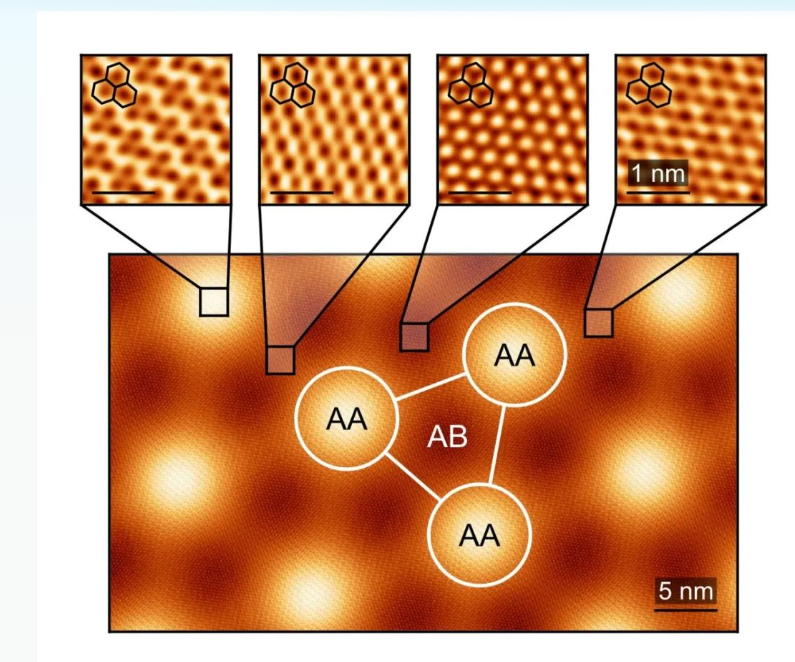
\includegraphics[scale=0.6]{figures/sm.png}
\end{figure}

\section{转角石墨烯实现超导}
单层石墨烯的许多性质都可以用自由电子的物理图像来定性地理解,在这个物理图像中电子之间的排斥作用被忽略掉了。例如,单层石墨烯中电子能量和动量的色散关系可以很好地近似为不依赖于周围电子的密度。“魔角”双层石墨烯的情况则截然不同(最大魔角大概为1度)。在这种情况下,电子会占据平带(平带也就是很平的能带)。由于这些平带的带宽很小,电子之间的相互作用不能再当做微扰来处理,这时候系统的物理性质就会强烈依赖于电子密度。这种强相互作用甚至会引起单层石墨烯中没有的物相:在特定的电子密度下,虽然在自由电子物理图像中系统应该是金属,但是实际系统表现为绝缘体;并且,就像高温超导体一样,这时候增加或减少电子密度会减小电阻并出现超导(电阻为零)。

2018年nature为我们带来了两篇转角石墨烯超导的论文。根据1957年的超导电性理论,某些材料能够以零电阻导电。然而,许多材料表现出所谓的非常规超导电性,无法用该理论解释。美国麻省理工学院科学家帕博罗·加力罗-埃雷拉及其同事发现,当两层石墨烯以一个“神奇角度”缠扭在一起时,它们表现出非常规超导电性。也就是说,研究团队在两层石墨烯中发现了新的电子态,其可以简单实现绝缘体到超导体的转变,而其属性与铜氧化物(其结构往往难以调整)的高温超导类似。

这种“神奇角度”的石墨烯除了会形成超导态——来源于电子之间的强吸引作用而产生零电阻,还会形成另一种电子态。在第二篇论文中,该团队展示了缠扭的双层石墨烯系统会出现一种新的绝缘态——莫特绝缘体态(Mott Insulator),这种状态似乎由强大的电子间相互作用推动产生。两篇论文所报告的系统,可以通过改变扭转角度和电场来轻易调整。这意味着,该成果将提供一个全新的二维平台,以供科学家们理解曾长期困扰物理学界的高温超导电性的起源问题,并将打开一扇研究非常规超导体的大门,同时也为全新电学性能的开拓和工程化铺平道路。

此外,转角石墨烯之所以吸引着无数研究人员,还因为其掺杂后变成Mott绝缘体再变成超导体的相图和常规的高温金属超导体一模一样,但这些材料均是块体材料,而石墨烯仅仅是二维材料,这对物理学来说无疑是反常的,人们都希望通过石墨烯来了解高温超导的机理,目前这项工作还未有较大的进展,但依旧吸引着无数科学家攀登着这座高峰

\section{未来的应用}
由于转角石墨烯存在超导的可能性,未来的应用变得十分的广泛,比如:交通应用。磁悬浮列车利用超导材料的抗磁性实现悬浮和高速运行,减少摩擦,提高运行效率。电力应用。超导电缆可以减少电能传输过程中的损耗,提高电力传输效率。超导发电机和电机制造利用超导体的零电阻特性产生强磁场,提高电力输出和效率。医学应用。超导核磁共振成像(MRI)设备使用超导磁体产生强磁场,提高成像分辨率和灵敏度,用于医学诊断。电子学和计算机应用。超导量子干涉器(SQUID)等电子器件用于测量非常微弱的磁场,提高测量精度。超导计算机使用超导器件减少散热问题,提高运算速度。科学研究应用。高能粒子加速器和核聚变装置使用超导磁体产生强磁场,加速粒子或控制核聚变反应。能源储存和应用。超导储能系统能够长时间、大容量地储存能量,用于军事上的聚能武器或民用领域的能源储存。其他应用。超导技术还应用于生物传感器、量子计算、航空航天等领域,提高相关技术的性能和效率。

此外石墨烯现在也广泛用于了太阳能电池和传感器中,石墨烯可以作为透明导电薄膜,在太阳能电池中起到了关键作用。石墨烯的界面处分离光生载流子,可以与传统硅材料结合,推动基于石墨烯的光伏器件的发展。此外,石墨烯也可以用于制造锂离子电池,同时也可以用于储能系统。石墨烯的储电量也是市场最好产品的三倍,是锂离子电池的两倍。这些但表面了石墨烯的未来具有无限的研究潜力。
\



\section*{参考文献}

1. Cao, Y. et al. Nature 556, 43–50 (2018).

2. Cao, Y. et al. Nature 556, 80–84 (2018).

3. Kerelsky, A. et al. Nature 572, 95–100 (2019).

4. Xie, Y. et al. Nature 572, 101–105 (2019).

5. Jiang, Y. et al. Nature https://doi.org/10.1038/s41586-019-1460-4 (2019).

6. Choi, Y. et al. Preprint at https://arxiv.org/abs/1901.02997 (2019).

7. Bistritzer, R. MacDonald, A. H. Proc. Natl Acad. Sci.USA108, 12233–12237 (2011).

8. Shen, C. et al. Preprint at https://arxiv.org/abs/1903.06952 (2019).

9.Liu, X. et al. Preprint at https://arxiv.org/abs/1903.08130 (2019).

10.Cao, Y. et al. Preprint at https://arxiv.org/abs/1903.08596 (2019).


\end{document}